\documentclass[11pt,a4paper]{article}

% ===================== Codificación y fuentes =====================
\usepackage[utf8]{inputenc}
\usepackage[T1]{fontenc}

% ===================== Página y utilidades ========================
\usepackage[left=2.5cm,right=2.5cm,top=2.5cm,bottom=2.5cm]{geometry}
\usepackage{array}
\usepackage{enumitem}
\usepackage{graphicx}
\usepackage{float}
\usepackage{xcolor}
\usepackage{titlesec}
\usepackage{fancyhdr}
\usepackage[most]{tcolorbox}
\usepackage{hyperref}
\usepackage{booktabs}

% ===================== Etiquetas en español (sin babel) ===========
\renewcommand{\contentsname}{Índice}
\renewcommand{\figurename}{Figura}
\renewcommand{\tablename}{Tabla}
\renewcommand{\refname}{Bibliografía}

% ===================== Escala de grises (sin color) ================
\definecolor{negro}{RGB}{0,0,0}
\definecolor{gris}{RGB}{90,90,90}
\definecolor{grisclaro}{RGB}{150,150,150}
\definecolor{fillgray}{RGB}{175,175,175}

% ===================== Hipervínculos (negro) =======================
\hypersetup{colorlinks=true, linkcolor=negro, urlcolor=negro, citecolor=negro}

% ===================== Estilo de títulos ===========================
\titleformat{\section}{\large\bfseries\color{negro}}{\thesection.}{0.5em}{}
\titleformat{\subsection}{\normalsize\bfseries\color{negro}}{\thesubsection}{0.5em}{}
\titlespacing*{\section}{0pt}{1.4em}{0.4em}
\titlespacing*{\subsection}{0pt}{1.0em}{0.3em}

% ===================== Pie de página ===============================
\pagestyle{fancy}
\fancyhf{}
\fancyfoot[L]{\footnotesize\color{gris}Magíster en Ciencia de Datos e Inteligencia Artificial}
\fancyfoot[R]{\footnotesize\color{gris}\thepage}
\renewcommand{\headrulewidth}{0pt}
\renewcommand{\footrulewidth}{0.4pt}

% Caja de información de la evaluación (escala de grises):
\newtcolorbox{infobox}[1][Información de la evaluación]{colback=black!3,colframe=negro,
  fonttitle=\bfseries,coltitle=white,title={#1},boxrule=0.6pt,arc=1pt,
  left=8pt,right=8pt,top=6pt,bottom=6pt,breakable}

% ===================== Datos del grupo ==============================
\newcommand{\proyTitulo}{Predicción de riesgo de enfermedad coronaria a 10 años}
\newcommand{\proyIntegrantes}{Felipe Díaz Toro, Pablo Ríos Passteni, Guillermo Subiabre Chacón, Ninoska Yévenes Hernández}
\newcommand{\proyDataset}{Framingham Heart Study (Riesgo Cardiovascular)}
\newcommand{\proyDocente}{Jean Paul Maidana}
\newcommand{\proyFecha}{09/10/2026}
\newcommand{\proyRepo}{\url{https://github.com/fdiaztoro/proyecto-grupo3-mcdi501}}

\setlength{\parindent}{0pt}
\setlength{\parskip}{0.35em}

\begin{document}
\pagenumbering{gobble}

\thispagestyle{empty}
\begin{center}
\vspace*{1.0cm}

\includegraphics[height=4.4cm]{logo_unab.png}\\[1.3cm]

{\footnotesize\color{gris}\MakeUppercase{Magíster en Ciencia de Datos e Inteligencia Artificial}}\\[0.15cm]
{\footnotesize\color{grisclaro}MCDI501: Estadística Computacional para la Toma de Decisiones}\\[2.0cm]

{\Large\bfseries\color{negro} Evaluación Sumativa 1}\\[0.45cm]
{\large\color{negro} Análisis Exploratorio e Inferencial}\\[1.0cm]

{\LARGE\bfseries\color{negro} \proyTitulo}\\[0.4cm]
{\normalsize\color{gris} Framingham Heart Study}\\[0.8cm]

{\small\itshape\color{gris} Informe técnico grupal \textperiodcentered\ Grupo 3 \textperiodcentered\ 20\,\%}
\end{center}

\vspace{1.6cm}

\begin{flushleft}
\setlength{\extrarowheight}{5pt}
\begin{tabular}{@{}>{\bfseries\color{negro}}l >{\raggedright\arraybackslash}p{11cm}@{}}
Título del proyecto: & \proyTitulo \\
Integrantes:         & \proyIntegrantes \\
Dataset:             & \proyDataset \\
Docente:             & \proyDocente \\
Fecha:               & \proyFecha \\
Repositorio GitHub:  & \proyRepo \\
\end{tabular}
\end{flushleft}

\clearpage
\pagenumbering{arabic}
\begin{infobox}
\textbf{Fase del proyecto:} Fase 2: Búsqueda y recopilación de información\\
\textbf{Modalidad:} Grupal (3--4 integrantes)\qquad\textbf{Ponderación:} 20\,\% de la nota final\\
\textbf{Entregables:} Informe PDF (máx.\ 8 págs., sin anexos) \ \textperiodcentered\ Notebook \texttt{.ipynb}\ \textperiodcentered\ Repositorio GitHub\\
\textbf{Resultado de aprendizaje (RA1):} aplicar probabilidad e inferencia estadística en problemas de decisión bajo incertidumbre.\\
\textbf{Indicadores:} ID1.2, ID1.3, ID1.4.\\
\textbf{Recuerden:} los resultados de esta sumativa serán la entrada de S2 y S3.
\end{infobox}

\vspace{0.5em}
\tableofcontents

% =====================================================================
\section{Preparación y carga de datos}

El proyecto utiliza la versión pública en Kaggle del \textbf{Framingham Heart Study} (Dileep, s.f.),
uno de los estudios de cohorte cardiovascular más influyentes (Mahmood et~al., 2014). Reúne
\textbf{4.238 participantes} y 16 variables: la variable objetivo \texttt{TenYearCHD}, que indica si la
persona desarrolló \textbf{enfermedad coronaria (CHD) en los diez años siguientes}, y 15 predictores
medidos al inicio del seguimiento. El conjunto se carga en Python con \texttt{kagglehub} y
\texttt{pandas}; todas las columnas llegan como numéricas, pero corresponden a seis indicadores binarios
(sexo, fumador actual, medicación antihipertensiva, ACV previo, hipertensión prevalente y diabetes), una
variable ordinal (nivel educativo, 1 a 4), un conteo (cigarrillos por día) y siete variables numéricas
(edad, colesterol total, presión sistólica y diastólica, IMC, frecuencia cardíaca y glucosa).

La revisión de calidad muestra un conjunto limpio en estructura. No hay filas duplicadas ni
inconsistencias entre variables relacionadas: ninguna presión diastólica iguala o supera a la sistólica,
el hábito de fumar es coherente con los cigarrillos por día y las binarias solo toman los valores 0 y 1.
Hay \textbf{datos faltantes en siete variables} (Figura~\ref{fig:panorama}b): la glucosa concentra 388
(9{,}2\,\%) y el nivel educativo 105 (2{,}5\,\%); el resto no supera el 1{,}3\,\%. En total, 582 filas
(13{,}7\,\%) tienen al menos un faltante. Para orientar su tratamiento se comparó la tasa de CHD con y sin
dato de glucosa: la diferencia no es significativa ($\chi^2=1{,}58$; $p=0{,}21$), un indicio de que la
pérdida no depende del desenlace. Los valores extremos según la regla de Tukey van de 1{,}3\,\%
(colesterol) a 4{,}9\,\% (glucosa) de las observaciones y son clínicamente plausibles: los 34 registros con
glucosa de 200 mg/dL o más corresponden todos a personas diabéticas. La Tabla~\ref{tab:limpieza}
documenta las decisiones.

\begin{table}[H]
\centering
\small
\caption{Decisiones de limpieza y tratamiento de datos.}
\label{tab:limpieza}
\begin{tabular}{>{\raggedright\arraybackslash}p{4.6cm} >{\raggedright\arraybackslash}p{10.2cm}}
\toprule
\textbf{Situación} & \textbf{Decisión} \\
\midrule
Faltantes en 7 variables (13{,}7\,\% de las filas) & Se trabaja con los casos disponibles de cada variable; la imputación se aborda en el modelamiento. \\
Glucosa faltante (9{,}2\,\%) & No se asocia con CHD ($p=0{,}21$); se usan los casos con dato. \\
Cigarrillos por día faltantes (29) & Los 29 son fumadores actuales; podrán imputarse con la mediana de los fumadores. \\
Valores extremos (Tukey) & Se conservan por ser plausibles (glucosa $\geq200$ solo en diabéticos); se usa la mediana como referencia y en los gráficos se recorta la cola solo para visualizar. \\
Duplicados e inconsistencias & No se detectaron; no requieren tratamiento. \\
\bottomrule
\end{tabular}
\end{table}

% =====================================================================
\section{Análisis exploratorio de datos}

\subsection{Estadística descriptiva}
La Tabla~\ref{tab:descriptivos} resume las variables numéricas. La edad es la única casi simétrica
(media 49{,}58, mediana 49 y asimetría 0{,}23). El colesterol, la presión sistólica y el IMC tienen asimetría
moderada a la derecha, con la media por sobre la mediana, y la glucosa es la más sesgada (6{,}21), arrastrada
por los valores altos de las personas diabéticas. En cigarrillos por día la mediana es 0 y la media 9: más
de la mitad no fuma y la media la elevan los fumadores intensos.

\begin{table}[H]
\centering
\small
\caption{Medidas descriptivas de las variables numéricas (casos disponibles de cada variable).}
\label{tab:descriptivos}
\setlength{\tabcolsep}{4.5pt}
\begin{tabular}{lrrrrrrr}
\toprule
\textbf{Variable} & \textbf{Media} & \textbf{Mediana} & \textbf{Desv. est.} & \textbf{Mín.} & \textbf{Máx.} & \textbf{Asimetría} & \textbf{$n$} \\
\midrule
Edad (años)                & 49{,}58  & 49{,}00  & 8{,}57  & 32       & 70       & 0{,}23 & 4.238 \\
Cigarrillos por día        & 9{,}00   & 0{,}00   & 11{,}92 & 0        & 70       & 1{,}25 & 4.209 \\
Colesterol total (mg/dL)   & 236{,}72 & 234{,}00 & 44{,}59 & 107      & 696      & 0{,}87 & 4.188 \\
Presión sistólica (mmHg)   & 132{,}35 & 128{,}00 & 22{,}04 & 83{,}5   & 295      & 1{,}15 & 4.238 \\
Presión diastólica (mmHg)  & 82{,}89  & 82{,}00  & 11{,}91 & 48       & 142{,}5  & 0{,}71 & 4.238 \\
IMC (kg/m$^2$)             & 25{,}80  & 25{,}40  & 4{,}08  & 15{,}54  & 56{,}8   & 0{,}98 & 4.219 \\
Frecuencia cardíaca (lpm)  & 75{,}88  & 75{,}00  & 12{,}03 & 44       & 143      & 0{,}64 & 4.237 \\
Glucosa (mg/dL)            & 81{,}97  & 78{,}00  & 23{,}96 & 40       & 394      & 6{,}21 & 3.850 \\
\bottomrule
\end{tabular}
\end{table}

Entre las variables categóricas (Tabla~\ref{tab:binarias}), el 42{,}9\,\% son hombres, el 49{,}4\,\% fuma
y el 31{,}1\,\% tiene hipertensión prevalente. La tasa de CHD es mayor en quienes tienen cada antecedente,
salvo el tabaquismo, que casi no la cambia. El nivel educativo se concentra en el nivel 1 (41{,}6\,\%), que
tiene además la mayor tasa de CHD (18{,}8\,\%). La variable objetivo está \textbf{desbalanceada}: 644
participantes (15{,}2\,\%) desarrollan CHD, unas 5{,}6 personas sanas por cada caso
(Figura~\ref{fig:panorama}a).

\begin{table}[H]
\centering
\small
\caption{Variables binarias: prevalencia y tasa de CHD a 10 años según el atributo.}
\label{tab:binarias}
\begin{tabular}{lrrr}
\toprule
\textbf{Variable} & \textbf{\% con atributo} & \textbf{\% CHD (con)} & \textbf{\% CHD (sin)} \\
\midrule
Sexo masculino               & 42{,}9 & 18{,}9 & 12{,}4 \\
Fumador actual               & 49{,}4 & 15{,}9 & 14{,}5 \\
Medicación antihipertensiva  & 3{,}0  & 33{,}1 & 14{,}6 \\
ACV previo                   & 0{,}6  & 44{,}0 & 15{,}0 \\
Hipertensión prevalente      & 31{,}1 & 24{,}7 & 10{,}9 \\
Diabetes                     & 2{,}6  & 36{,}7 & 14{,}6 \\
\bottomrule
\end{tabular}
\end{table}

\begin{figure}[H]
\centering
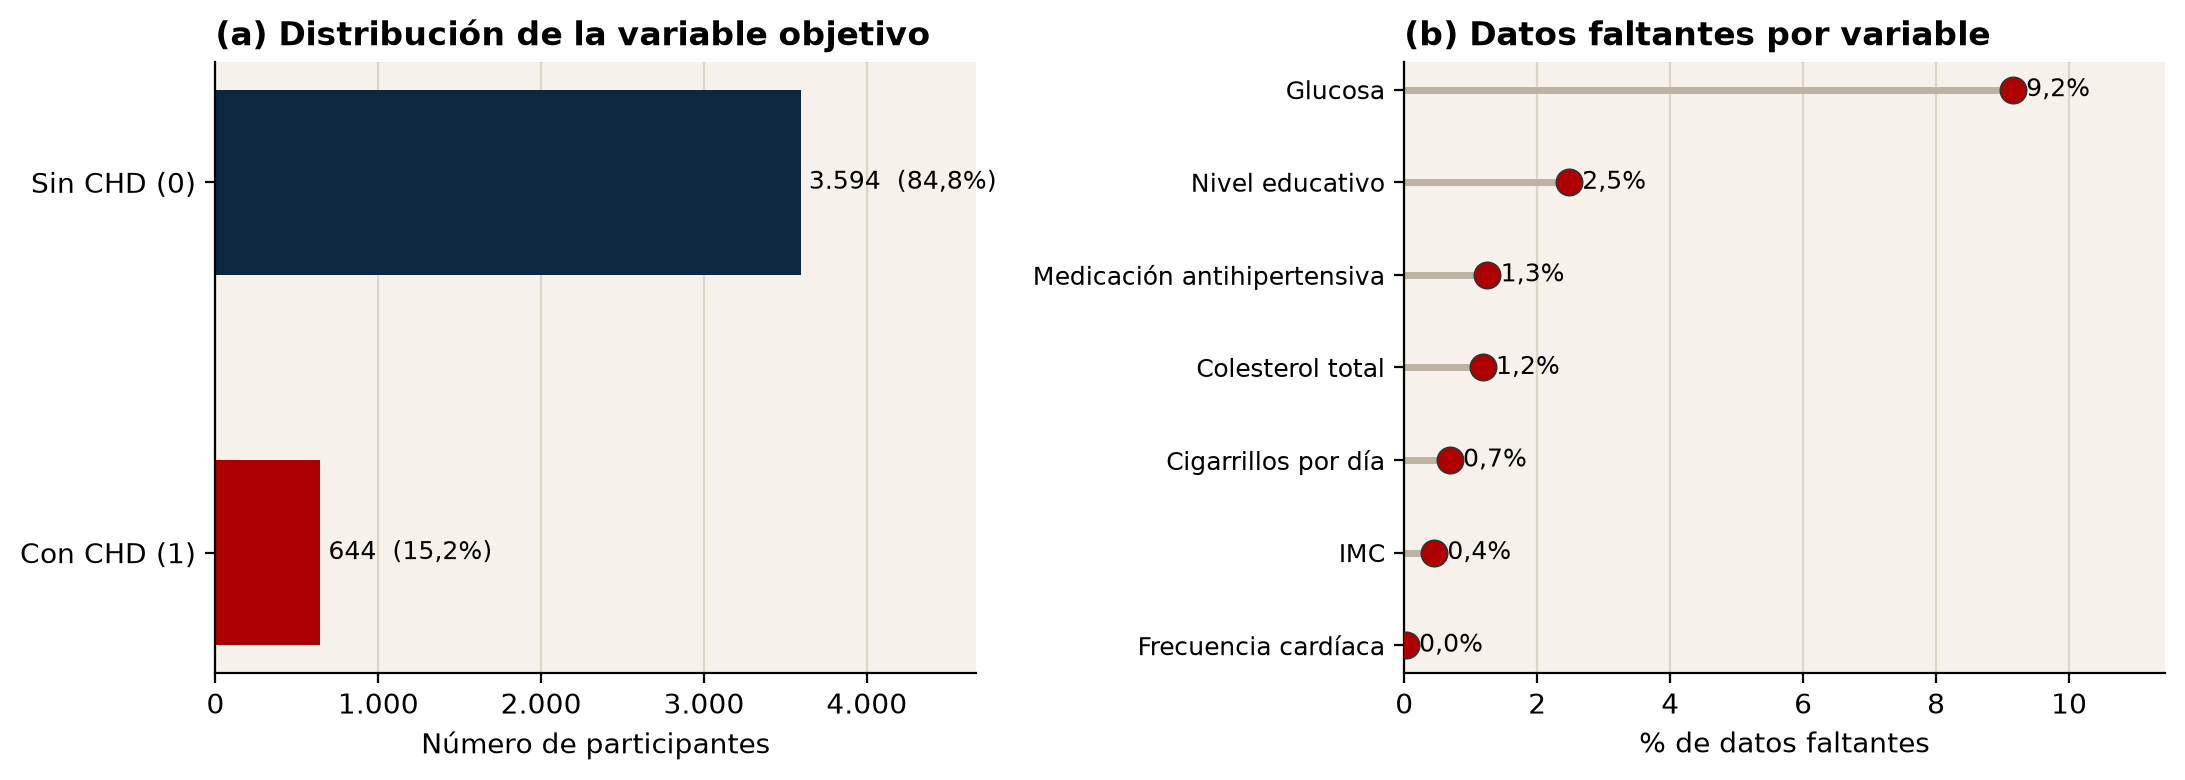
\includegraphics[width=0.92\linewidth]{figuras/fig_panorama.png}
\caption{(a) Distribución de la variable objetivo. (b) Porcentaje de datos faltantes por variable.}
\label{fig:panorama}
\end{figure}

La Figura~\ref{fig:distribuciones} confirma las formas: la edad se reparte de forma aproximadamente
simétrica en torno a 50 años, mientras que el colesterol y la presión sistólica tienen la mediana
(234 mg/dL y 128 mmHg) bajo la media y una cola de valores altos.

\begin{figure}[H]
\centering
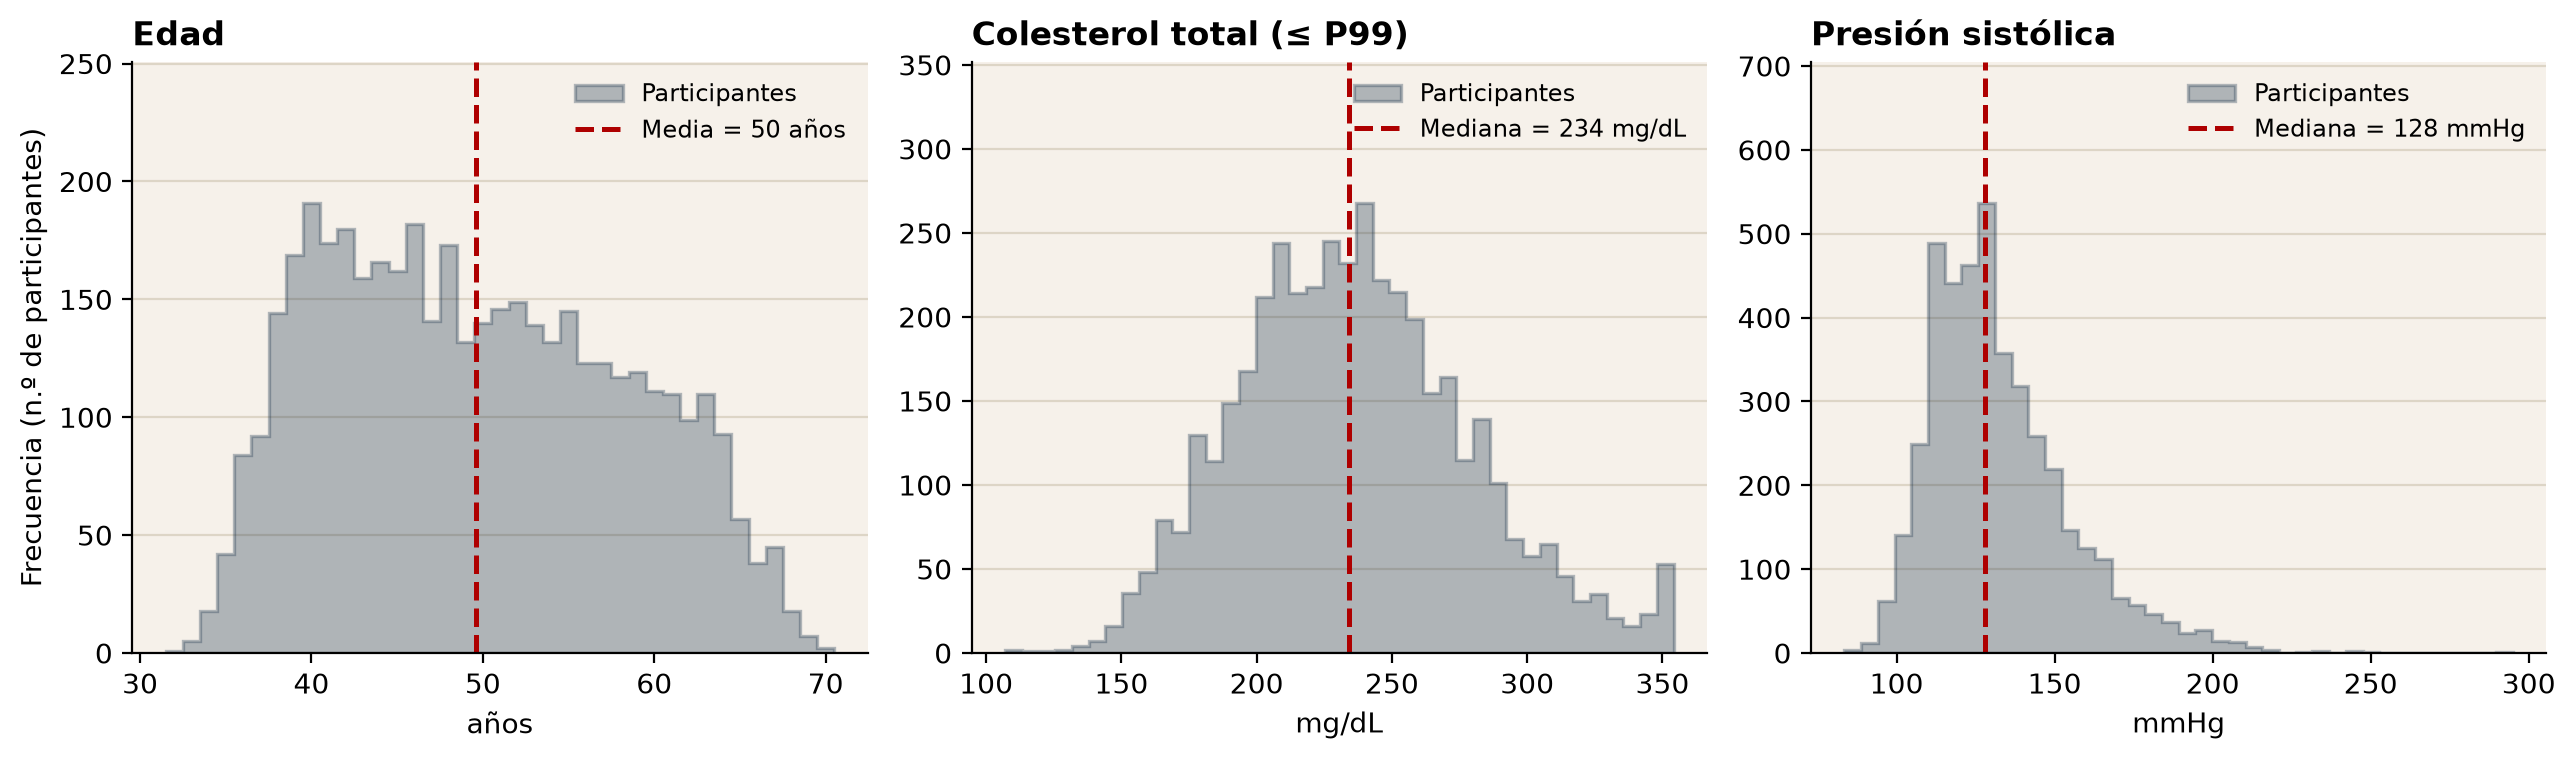
\includegraphics[width=\linewidth]{figuras/fig_distribuciones.png}
\caption{Distribución de tres variables numéricas, con su media o mediana de referencia (colesterol recortado al percentil 99 solo para visualizar).}
\label{fig:distribuciones}
\end{figure}

\subsection{Análisis bivariado}
La matriz de correlaciones (Figura~\ref{fig:correlacion}) muestra pares muy relacionados: presión sistólica
y diastólica ($r=0{,}78$), fumador actual y cigarrillos por día ($r=0{,}77$, en parte estructural),
hipertensión prevalente y presión sistólica ($r=0{,}70$) y diabetes y glucosa ($r=0{,}62$), lo que anticipa
colinealidad si se modelan juntos. Con el objetivo, todas las correlaciones lineales son débiles; las mayores
son la edad ($r=0{,}23$), la presión sistólica ($r=0{,}22$) y la hipertensión ($r=0{,}18$). Cuando una de las
variables es binaria, el coeficiente de Pearson equivale al punto biserial (binaria con numérica) o al
coeficiente phi (binaria con binaria).

\begin{figure}[H]
\centering
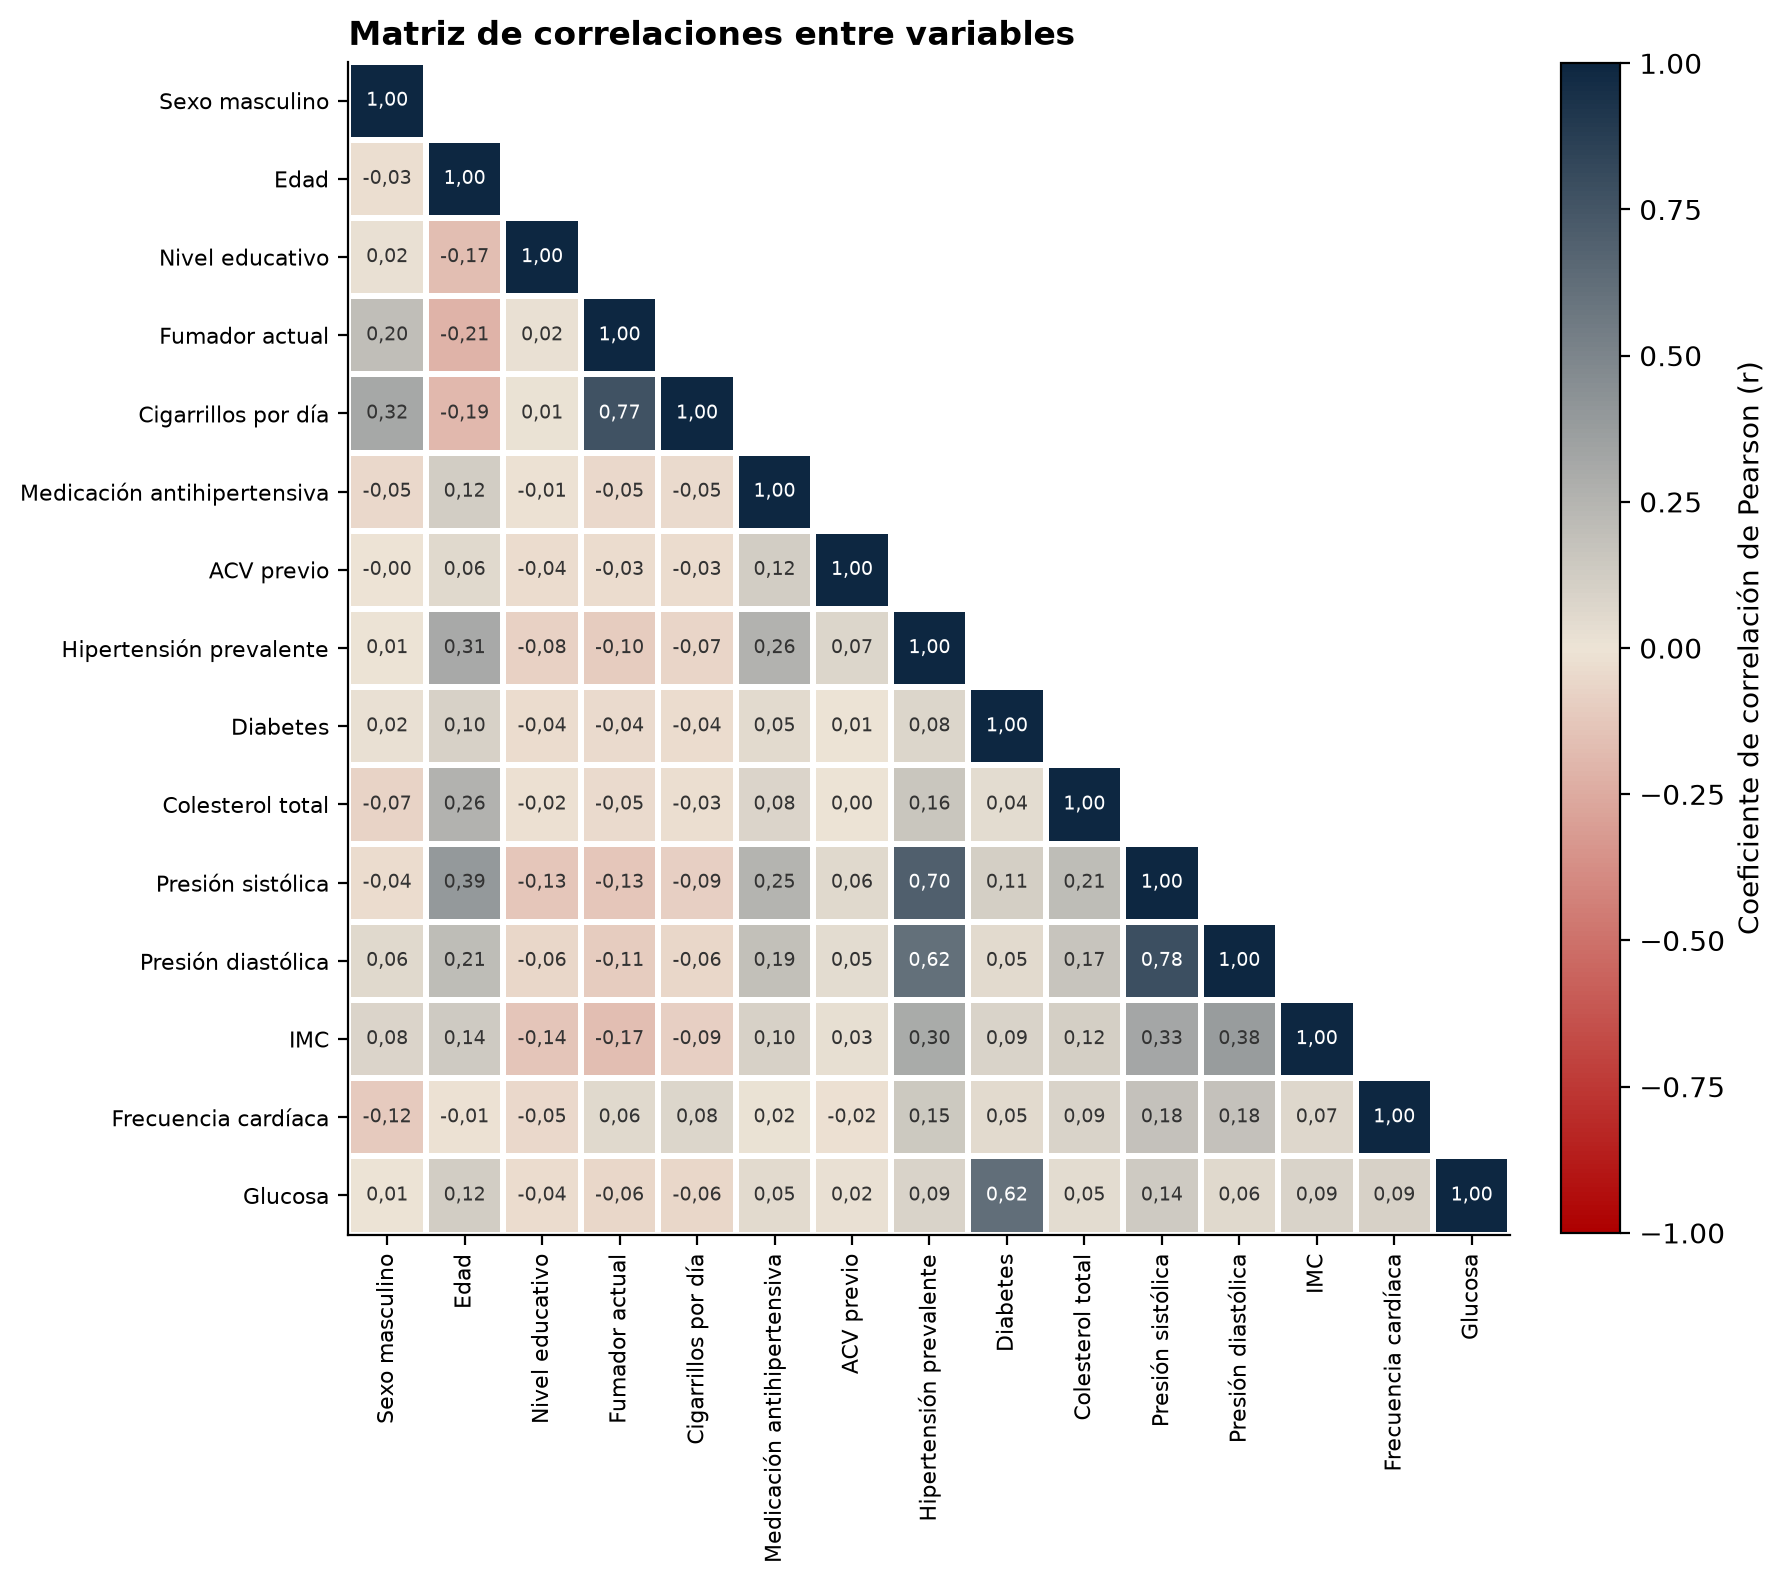
\includegraphics[width=0.66\linewidth,height=8.2cm,keepaspectratio]{figuras/fig_correlacion.png}
\caption{Matriz de correlaciones entre las variables predictoras (triángulo inferior).}
\label{fig:correlacion}
\end{figure}

Como la correlación resume mal la relación con un desenlace binario poco frecuente, se construyeron dos
variables categóricas: el tramo etario (decenios) y la categoría de presión sistólica, con cortes cercanos a
los umbrales clínicos (normal bajo 120 mmHg, elevada de 120 a 129 e hipertensión desde 130; Whelton et~al.,
2018). La Figura~\ref{fig:bivariado} muestra que la tasa de CHD crece de forma \textbf{monótona} con ambas:
del 4{,}1\,\% entre los 32 y 39 años al 27{,}7\,\% entre los 60 y 70 (casi siete veces más), y del 8{,}5\,\%
bajo 120 mmHg al 30{,}8\,\% desde 160 mmHg. Son relaciones mucho más marcadas de lo que sugieren sus
correlaciones, y señalan a la edad y la presión arterial como los ejes del riesgo.

\begin{figure}[H]
\centering
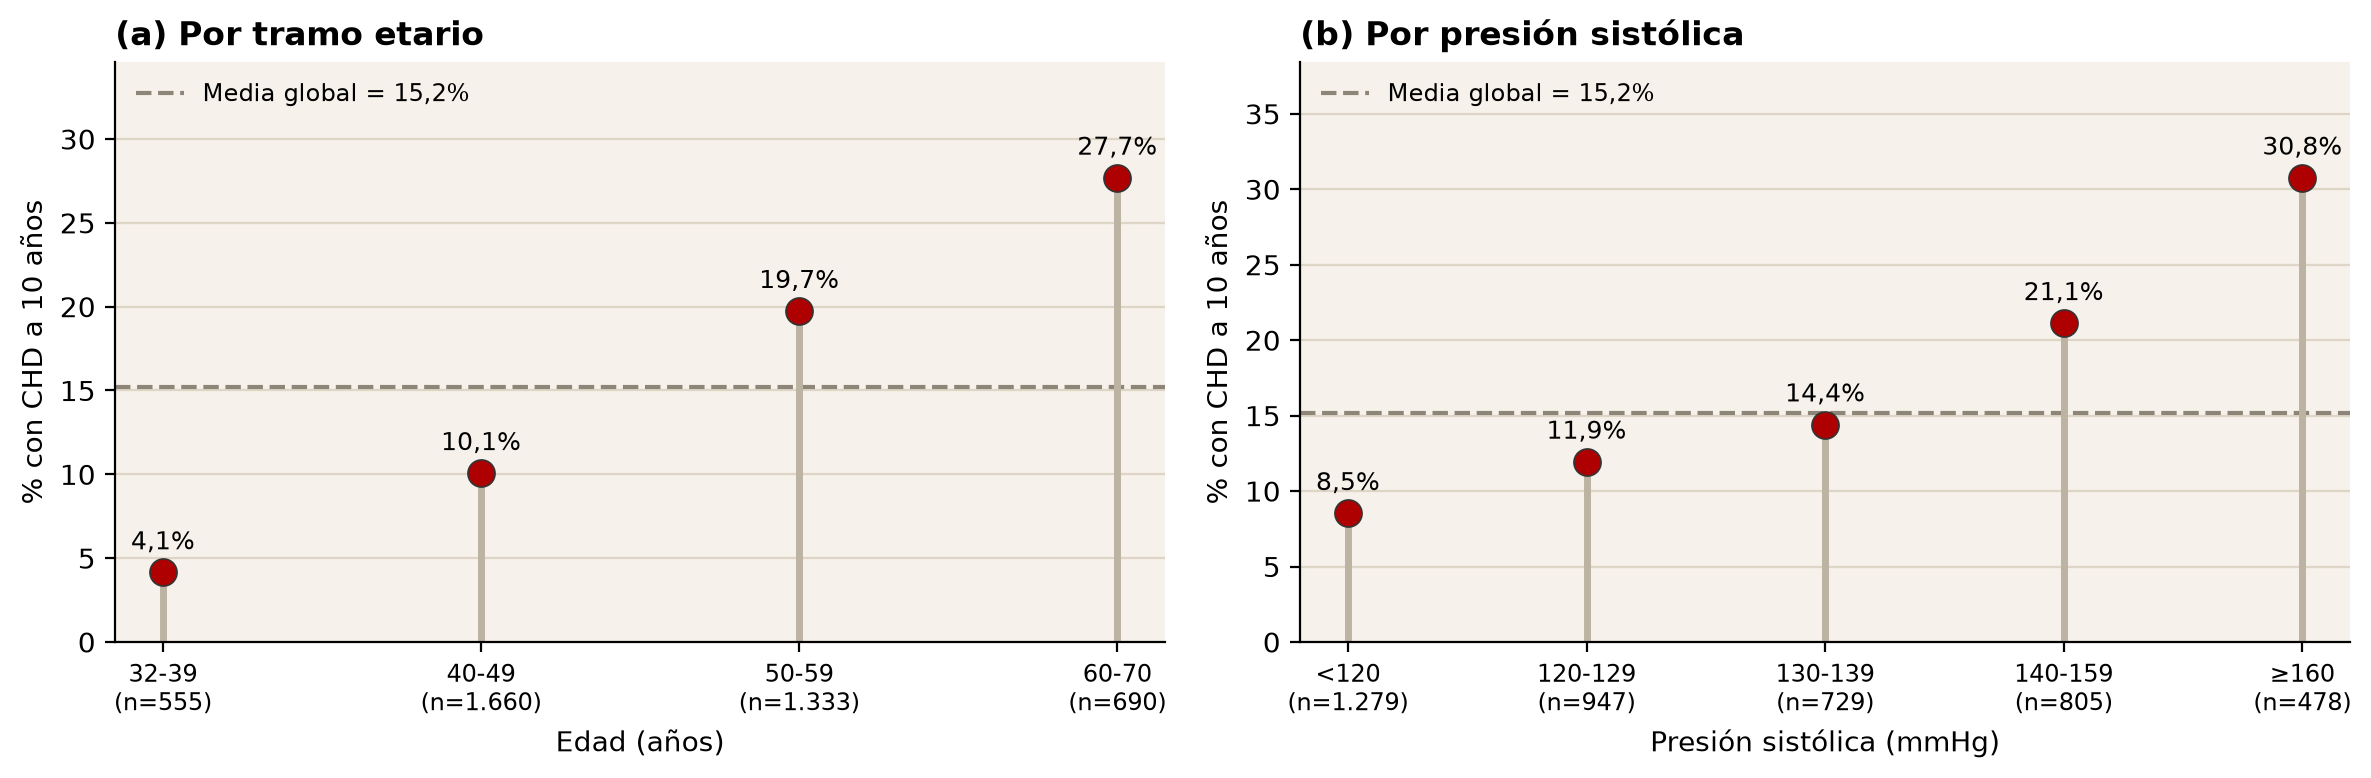
\includegraphics[width=\linewidth]{figuras/fig_bivariado.png}
\caption{Tasa de CHD a 10 años por tramo etario y por categoría de presión sistólica, con la media global de referencia.}
\label{fig:bivariado}
\end{figure}

% =====================================================================
\section{Estimación de parámetros}

Se estimaron cuatro parámetros poblacionales con un 95\,\% de confianza (Tabla~\ref{tab:ic}). Para las medias
de tres variables numéricas se usó el intervalo basado en la aproximación normal,
$\bar{x}\pm z_{0{,}975}\,EE$ con $EE=s/\sqrt{n}$, justificado por el Teorema Central del Límite dado el tamaño
de la muestra (Wasserman, 2004). Para la proporción de CHD se usó la misma aproximación (método de Wald),
$\hat{p}\pm z_{0{,}975}\sqrt{\hat{p}(1-\hat{p})/n}$. Cada intervalo usa los casos disponibles, sin imputar.

\begin{table}[H]
\centering
\small
\caption{Estimación puntual e intervalos de confianza al 95\,\%.}
\label{tab:ic}
\setlength{\tabcolsep}{4pt}
\begin{tabular}{lrcrrl}
\toprule
\textbf{Parámetro} & \textbf{Estimación} & \textbf{IC 95\,\%} & \textbf{Mediana} & \textbf{$n$} & \textbf{Método} \\
\midrule
Edad media (años)              & 49{,}58     & [49{,}33; 49{,}84]          & 49  & 4.238 & Normal (TCL) \\
Colesterol total medio (mg/dL) & 236{,}72    & [235{,}37; 238{,}07]        & 234 & 4.188 & Normal (TCL) \\
Presión sistólica media (mmHg) & 132{,}35    & [131{,}69; 133{,}02]        & 128 & 4.238 & Normal (TCL) \\
Proporción de CHD a 10 años    & 15{,}20\,\% & [14{,}12\,\%; 16{,}28\,\%]  & --  & 4.238 & Normal (Wald) \\
\bottomrule
\end{tabular}
\end{table}

Los intervalos son estrechos por el tamaño muestral. Con un 95\,\% de confianza, la edad media poblacional
está entre 49{,}33 y 49{,}84 años, la presión sistólica media entre 131{,}69 y 133{,}02 mmHg y la proporción
de personas que desarrollan CHD a 10 años entre 14{,}12\,\% y 16{,}28\,\%; el intervalo de Wilson, alternativa
para proporciones, prácticamente coincide ([14{,}15\,\%; 16{,}31\,\%]).

La estimación tiene \textbf{limitaciones} que conviene declarar. El colesterol y la presión sistólica son
asimétricos: el TCL respalda la normalidad de la \textit{media muestral}, pero la media queda por sobre el
valor típico, por eso se informa también la mediana. El colesterol se estimó sin 50 casos faltantes
(1{,}2\,\%); si la pérdida no fuera aleatoria podría introducir un sesgo, aunque pequeño. Por último, los
intervalos suponen que la muestra representa a la población de interés, y la cohorte proviene de una sola
ciudad de Estados Unidos, por lo que la generalización debe hacerse con cautela.

% =====================================================================
\section{Pruebas de hipótesis}

Se aplicaron tres pruebas con nivel de significancia $\alpha=0{,}05$, valor habitual en estudios aplicados
que equilibra los errores de tipo I y II, eligiendo el procedimiento según el tipo de variable. El tamaño del
efecto se interpreta con los criterios de Cohen (1988).

\subsection{Prueba 1: diferencia de edad entre quienes desarrollan CHD y quienes no}
$$H_0:\ \mu_{\text{CHD}} = \mu_{\text{no CHD}} \qquad \text{vs.} \qquad H_1:\ \mu_{\text{CHD}} \neq \mu_{\text{no CHD}}$$
\textbf{Supuestos.} Los grupos son independientes, la edad es aproximadamente simétrica en ambos (asimetría
de $-0{,}25$ y $0{,}32$) y, con 644 y 3.594 personas, el TCL respalda la prueba \textit{t}. Como los tamaños son
muy dispares, se usa la prueba \textit{t} de Welch, que no asume varianzas iguales (Welch, 1947); la prueba de
Levene no detecta diferencia de varianzas al 5\,\% ($p=0{,}053$) y la \textit{t} de Student lleva a la misma
decisión ($t=15{,}05$).

\textbf{Resultado.} La edad media es 54{,}15 años en quienes desarrollan CHD y 48{,}77 en quienes no, una
diferencia de 5{,}38 años (IC 95\,\%: 4{,}70 a 6{,}06). El estadístico es $t=15{,}58$ con $p<0{,}001$, de modo
que \textbf{se rechaza $H_0$}, con un efecto moderado ($d$ de Cohen $=0{,}64$; Figura~\ref{fig:hipotesis}a).
La edad es un marcador de riesgo relevante, pero por sí sola no separa nítidamente a ambos grupos.

\subsection{Prueba 2: asociación entre hipertensión prevalente y CHD}
$$H_0:\ \text{hipertensión prevalente y CHD son independientes} \qquad \text{vs.} \qquad H_1:\ \text{están asociadas}$$
\textbf{Supuestos.} Se usa la prueba $\chi^2$ de independencia sobre una tabla de $2\times2$ con observaciones
independientes; la frecuencia esperada mínima es 200, muy por encima del umbral de 5.

\textbf{Resultado.} El 24{,}7\,\% de quienes tienen hipertensión desarrolla CHD, frente al 10{,}9\,\% de quienes
no (Figura~\ref{fig:hipotesis}b). La asociación es significativa ($\chi^2=132{,}6$; gl $=1$; $p<0{,}001$), por
lo que \textbf{se rechaza $H_0$}, con intensidad débil ($V$ de Cramér $=0{,}18$). El riesgo relativo es de 2{,}26
y la razón de momios de 2{,}68: la hipertensión más que duplica el riesgo y es un criterio simple y accionable
para priorizar el seguimiento.

\subsection{Prueba 3: asociación entre sexo y CHD}
$$H_0:\ \text{sexo y CHD son independientes} \qquad \text{vs.} \qquad H_1:\ \text{están asociados}$$
\textbf{Supuestos.} Prueba $\chi^2$ de independencia sobre una tabla de $2\times2$; la frecuencia esperada
mínima es 276, por lo que el supuesto se cumple.

\textbf{Resultado.} El 18{,}9\,\% de los hombres desarrolla CHD, frente al 12{,}4\,\% de las mujeres. La
asociación es significativa ($\chi^2=32{,}6$; gl $=1$; $p<0{,}001$), por lo que \textbf{se rechaza $H_0$}, aunque
con intensidad muy débil ($V=0{,}09$; riesgo relativo de 1{,}52 y razón de momios de 1{,}64). La diferencia no se
explica por la edad ni por la hipertensión, que son prácticamente iguales entre sexos (49{,}3 frente a 49{,}8
años; 31{,}3\,\% frente a 30{,}8\,\%). El sexo aporta una señal propia, más débil que la edad o la hipertensión.

\begin{figure}[H]
\centering
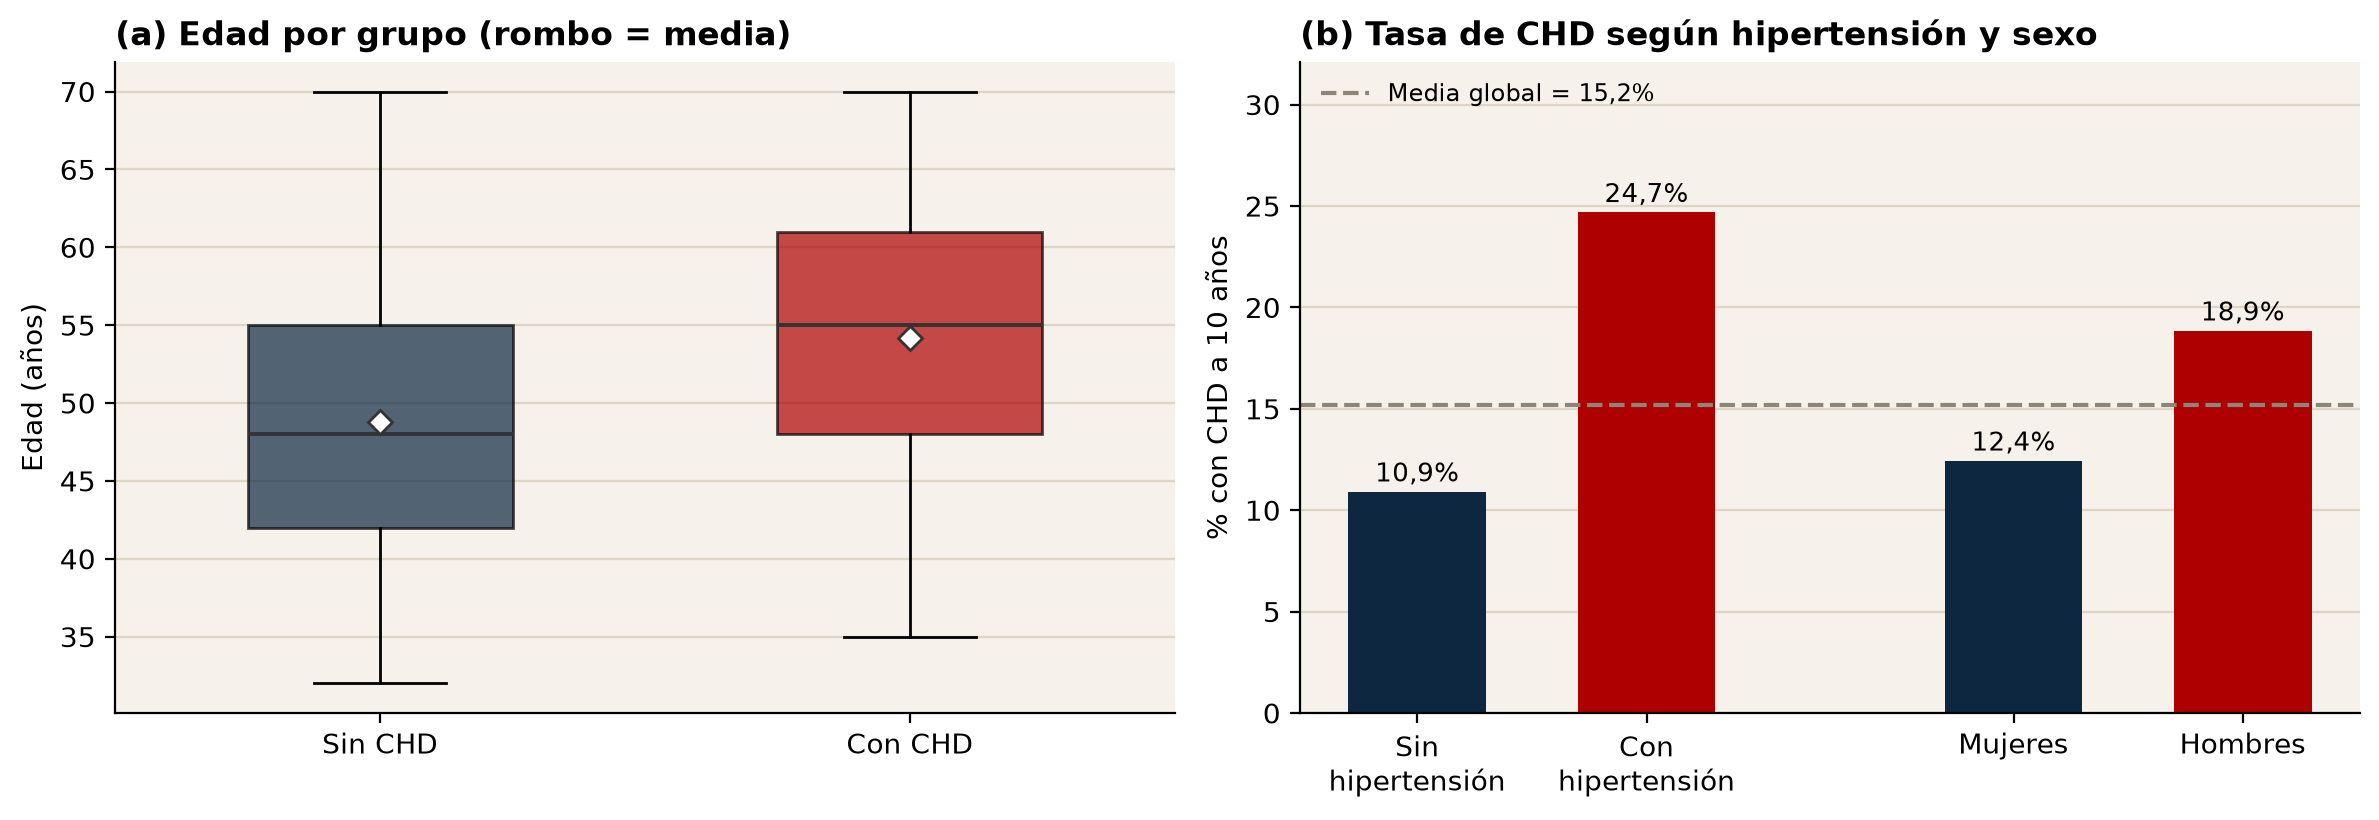
\includegraphics[width=\linewidth]{figuras/fig_hipotesis.png}
\caption{(a) Distribución de la edad por grupo (rombo: media). (b) Tasa de CHD a 10 años según hipertensión prevalente y sexo.}
\label{fig:hipotesis}
\end{figure}

% =====================================================================
\section{Informe de avance del proyecto}

El problema es de decisión bajo incertidumbre: anticipar, en atención primaria, qué personas tienen mayor
probabilidad de desarrollar enfermedad coronaria en diez años, para priorizar su control y prevención. En esta
fase se revisó la calidad de los datos y se documentó su tratamiento, se caracterizó el conjunto con
estadística descriptiva y gráficos según el tipo de variable, se exploraron relaciones bivariadas con
variables derivadas, se estimaron parámetros con intervalos de confianza y se contrastaron tres hipótesis
con la prueba \textit{t} de Welch y la prueba $\chi^2$ de independencia. Estos resultados profundizan los de la
Formativa 1 y son coherentes con ellos.

Los resultados ofrecen tres lecturas. La \textbf{edad} y la \textbf{presión arterial} son las señales más
claras: el riesgo crece de forma monótona con ambas y la hipertensión más que duplica la probabilidad de CHD.
El \textbf{sexo masculino} aporta una señal adicional, más débil. En cambio, el tabaquismo casi no se asocia
con el desenlace de forma aislada. Como advertencias, el desbalance del objetivo (15{,}2\,\%) exigirá evaluar
los modelos con métricas sensibles a la clase minoritaria y no solo con la exactitud, y la colinealidad entre
presión sistólica, diastólica e hipertensión obliga a no incluirlas juntas sin más. Los datos son
observacionales, por lo que las asociaciones no implican causalidad.

Los \textbf{próximos pasos} son imputar los faltantes (glucosa, nivel educativo y cigarrillos por día en
fumadores), evaluar el efecto de los valores extremos, validar las estimaciones mediante remuestreo en la
Sumativa 2 y entrenar modelos de clasificación en la Sumativa 3.

% =====================================================================
\section{Notebook y repositorio GitHub}

Todo el análisis se realizó en Python con \texttt{pandas} (McKinney, 2010), \texttt{numpy} (Harris et~al.,
2020), \texttt{scipy} (Virtanen et~al., 2020) y \texttt{matplotlib} (Hunter, 2007). El cuaderno
\texttt{Sumativa1\_\allowbreak FraminghamHeartStudy\_\allowbreak Codigo.ipynb} sigue el mismo orden de este informe, descarga los
datos, genera todas las tablas y figuras aquí incluidas y fija la semilla 42 para asegurar la
reproducibilidad. El código y los informes de cada evaluación están en el repositorio enlazado en la portada.

% =====================================================================
\section{Bibliografía}

\begin{list}{}{\leftmargin=1.5em \itemindent=-1.5em \itemsep=0.25em \parsep=0pt}\small\raggedright
\item Cohen, J. (1988). \textit{Statistical power analysis for the behavioral sciences} (2.\textsuperscript{a} ed.). Lawrence Erlbaum Associates.
\item Dileep. (s.f.). \textit{Heart disease prediction using logistic regression} [Conjunto de datos]. Kaggle. \url{https://www.kaggle.com/datasets/dileep070/heart-disease-prediction-using-logistic-regression}
\item Harris, C. R., Millman, K. J., van der Walt, S. J., Gommers, R., Virtanen, P., Cournapeau, D., \dots\ Oliphant, T. E. (2020). Array programming with NumPy. \textit{Nature, 585}(7825), 357--362. \url{https://doi.org/10.1038/s41586-020-2649-2}
\item Hunter, J. D. (2007). Matplotlib: A 2D graphics environment. \textit{Computing in Science \& Engineering, 9}(3), 90--95. \url{https://doi.org/10.1109/MCSE.2007.55}
\item Mahmood, S. S., Levy, D., Vasan, R. S., \& Wang, T. J. (2014). The Framingham Heart Study and the epidemiology of cardiovascular disease: A historical perspective. \textit{The Lancet, 383}(9921), 999--1008. \url{https://doi.org/10.1016/S0140-6736(13)61752-3}
\item McKinney, W. (2010). Data structures for statistical computing in Python. En \textit{Proceedings of the 9th Python in Science Conference} (pp.~56--61). \url{https://doi.org/10.25080/Majora-92bf1922-00a}
\item Virtanen, P., Gommers, R., Oliphant, T. E., Haberland, M., Reddy, T., Cournapeau, D., \dots\ SciPy 1.0 Contributors. (2020). SciPy 1.0: Fundamental algorithms for scientific computing in Python. \textit{Nature Methods, 17}(3), 261--272. \url{https://doi.org/10.1038/s41592-019-0686-2}
\item Wasserman, L. (2004). \textit{All of statistics: A concise course in statistical inference}. Springer.
\item Welch, B. L. (1947). The generalization of ``Student's'' problem when several different population variances are involved. \textit{Biometrika, 34}(1--2), 28--35. \url{https://doi.org/10.1093/biomet/34.1-2.28}
\item Whelton, P. K., Carey, R. M., Aronow, W. S., Casey, D. E., Collins, K. J., Dennison Himmelfarb, C., \dots\ Wright, J. T. (2018). 2017 ACC/AHA/AAPA/ABC/ACPM/AGS/APhA/ASH/ASPC/NMA/PCNA guideline for the prevention, detection, evaluation, and management of high blood pressure in adults. \textit{Hypertension, 71}(6), e13--e115. \url{https://doi.org/10.1161/HYP.0000000000000065}
\end{list}

\end{document}
